\documentclass[12pt]{article}
\usepackage[english]{babel}
\usepackage{natbib}
\usepackage{url}
\usepackage[utf8x]{inputenc}
\usepackage{amsmath}
\usepackage{amsfonts}
\usepackage{color}
\usepackage{graphicx}
\graphicspath{{images/}}
\usepackage{parskip}
\usepackage{fancyhdr}
\usepackage{vmargin}
\usepackage{multicol}
\usepackage{tabularx}
\usepackage{makecell}
\usepackage{float}
\setmarginsrb{3 cm}{1 cm}{3 cm}{1 cm}{1 cm}{1.5 cm}{1 cm}{1.5 cm}
 
\title{HRI system of tutoring robot}                 % Title
\author{Horpynchenko, Dmytro \\ Xu, Wei \\ Senler, Ekin}                                                           % Author
\newcommand{\studentnumber}{1807584 \\ 1797103 \\ 1801499}
\date{\today}                                                                               % Date
 
\makeatletter
\let\thetitle\@title
\let\theauthor\@author
\makeatother
 
\pagestyle{empty}
\fancyhf{}
 
\lhead{\thetitle}
%\cfoot{\thepage}
 
\begin{document}
 
%%%%%%%%%%%%%%%%%%%%%%%%%%%%%%%%%%%%%%%%%%%%%%%%%%%%%%%%%%%%%%%%%%%%%%%%%%%%%%%%%%%%%%%%%
 
\begin{titlepage}
        \centering
    
\includegraphics[scale = 0.2]{images/sapienza_logo_only.png}\\[1.0 cm]  % University Logo
    \textsc{\LARGE Sapienza University of Rome}\\[2.0 cm]    % University Name
    \vspace{2cm}
        \textsc{\Large Human-Robot Interaction}\\[0.5 cm]                           % Course Name
        %\textsc{\large Analysis of the paper}\\[0.5 cm]                            % Course details
        \rule{\linewidth}{0.2 mm} \\[0.4 cm]
        { \huge \bfseries \thetitle}\\
        \rule{\linewidth}{0.2 mm} \\[1.5 cm]
 
        \begin{minipage}{0.4\textwidth}
               \begin{flushleft} \large
                       \emph{Authors:}\\
                       \theauthor
                       \end{flushleft}
                       \end{minipage}~
                       \begin{minipage}{0.4\textwidth}
                       \begin{flushright} \large
                       \emph{Student Numbers:} \\
                       \studentnumber
               \end{flushright}
        \end{minipage}\\[2 cm]
 
 
        \vfill
 
\end{titlepage}
 
%%%%%%%%%%%%%%%%%%%%%%%%%%%%%%%%%%%%%%%%%%%%%%%%%%%%%%%%%%%%%%%%%%%%%%%%%%%%%%%%%%%%%%%%%
 
\tableofcontents
\pagebreak
 
%%%%%%%%%%%%%%%%%%%%%%%%%%%%%%%%%%%%%%%%%%%%%%%%%%%%%%%%%%%%%%%%%%%%%%%%%%%%%%%%%%%%%%%%%
 
\pagebreak
 
\section{Introduction}
During the past decades, many researchers have studied the effectiveness of computer systems in tutoring tasks. James A. Kulik (2015)\cite{0034654315581420} reviewed the literature from the period and found the ITSs (intelligent tutoring systems) raise student performance well beyond the level of conventional classes and even beyond the level achieved by students instructed by human tutors. With the rising of researches in human-robot interactions, the effectiveness of a social robot in tutoring tasks is also being studied. 
\\
From a recent large-scale study\cite{8673077}, researchers found that the tutoring interactions consisting of a robot and a tablet didn't have an added value on effectiveness when teaching English vocabulary to young children English vocabulary comparing to scenarios with only a tablet. However, previous study shows that physically-present robot tutors do produce better learning gains than on-screen tutors\cite{Leyzberg_thephysical}. 
\\
Confidering previous studies and inspired by \cite{Park:2017:GGM:2909824.3020213}, we decided to explore other subjects of tutoring. As a result, tangram-like game (See Section \ref{sect_game_descr}) with a socially-interactive robot were designed to help children develop a growing mindset. Results showed in Section \ref{sect_exper} has proved that  interacting with a peer-like robot can help children promote the same mindset. 
 
\newpage
\section{Concept}
\subsection{Idea}
\label{sect_idea}
Similar to the setup in \cite{Park:2017:GGM:2909824.3020213} we designed a social-friendly tutoring robot that is able to autonomously provide a support to children with learning a material that prepared by their teacher. In this way we are able to simplify and entertain learning process for children meanwhile reduce workload for human teachers.
\\
As a tutoring agent we used a Pepper robot - a semi-humanoid robot, produced by SoftBank Robotics, which is able to interact with humans in a social way through voice, gestures and visual information showed on it's tablet (See Figure \ref{pepper}). It has rich communication functionality  such as text-to-speech and voice recognition, anthropomorphic-like embodiment with full control over it's joints, comprehensive list of predefined gestures, sonar sensors for distances measurement, multiple cameras with face detection support and many more that allows building complex human-responsive solutions.
\begin{figure}[!h]
\begin{center}
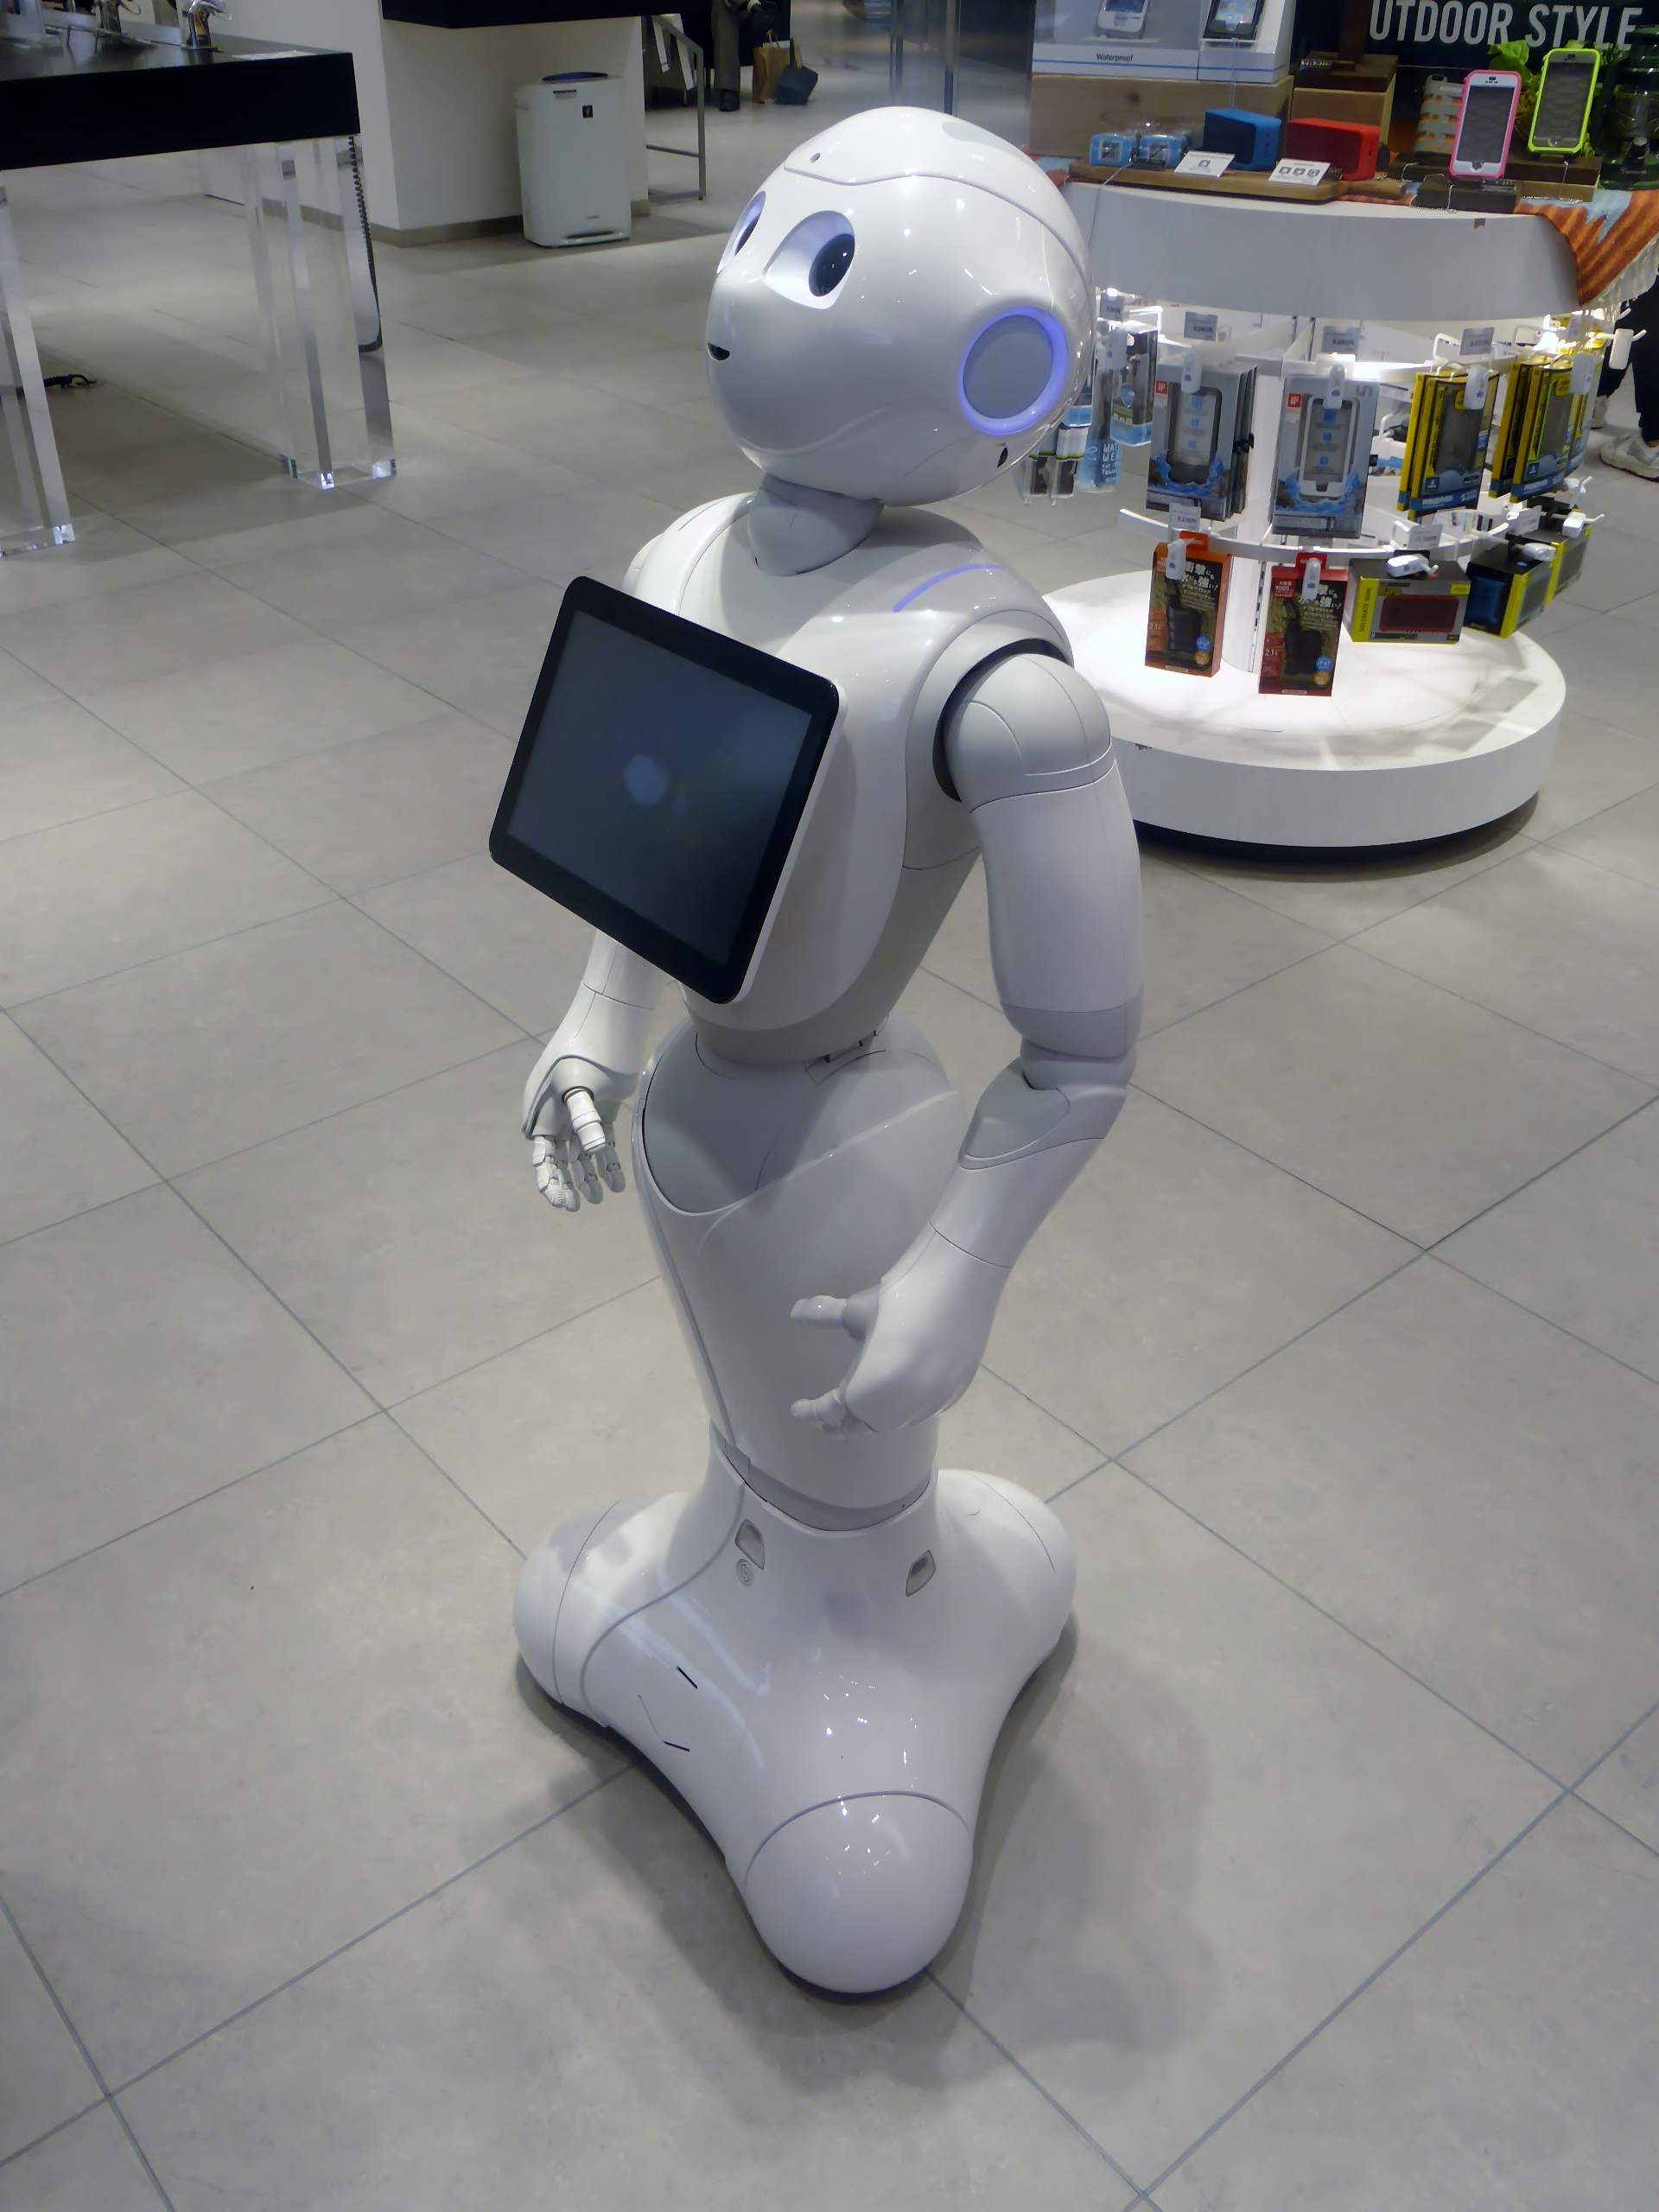
\includegraphics[scale=0.3]{images/pepper.jpg}
\caption{Pepper robot}
\label{pepper}
\end{center}
\end{figure}
\\
All tutoring process was established trough verbal communication supported by appropriate gestures from robot. On Figure \ref{concept_scheme} full robot-user interaction is shown. 
\\
First, robot introduce itself to peers such that to both explain it's mission and indicate it's readiness to use. Then it moves to the awaiting mode and observes space around for a person that is close enough and at the same time ready for communication.
\\
After detecting of the potential user Pepper offers him a practice of the cognitive skills and in case of positive answer will start game on it's tablet together with some little instructions. Behavior while user plays game more detailed described in the Section \ref{sect_game_descr}.
\\
After user finishes the game Pepper provides user with feedback regarding his results, like playing time in case of first round or time  improvement in comparing to the previous time. Here we might also give to user useful advises regarding improving playing techniques such that to receive progress in teaching and encourage kid for a new try. After  every round user is asked to play one more and depending from user answer will return to the awaiting mode or start game again.
\begin{figure}[!h]
\begin{center}
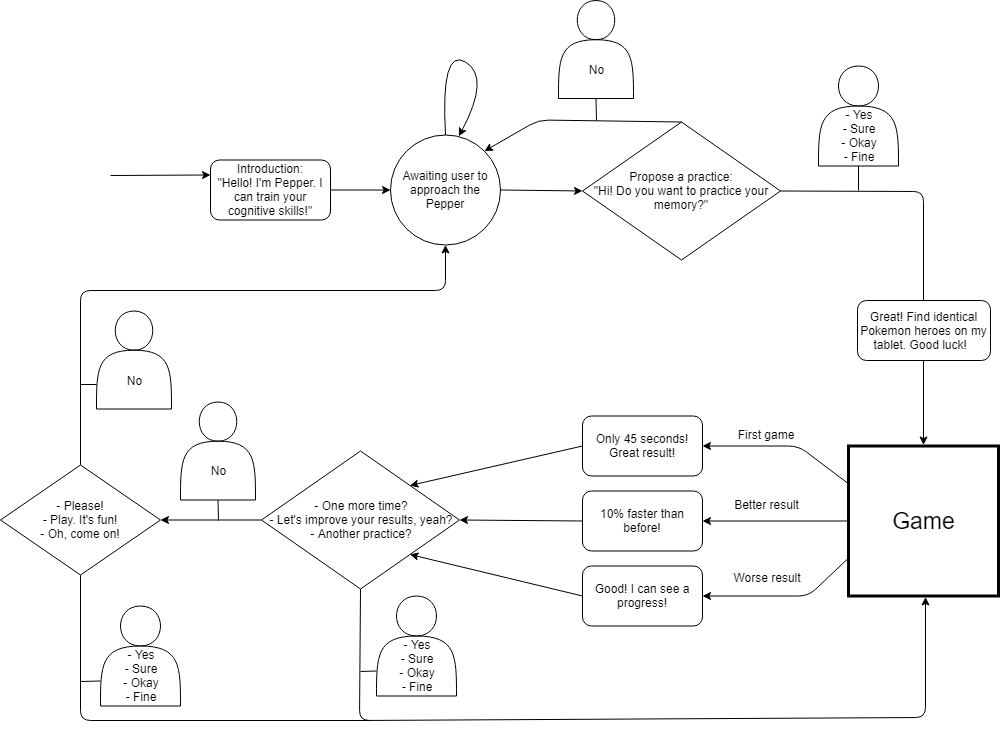
\includegraphics[scale=0.43]{images/HRI_concept.png}
\caption{Complex Pepper-User interaction scheme}
\label{concept_scheme}
\end{center}
\end{figure}
\subsection{Game}
\label{sect_game_descr}
We develop a memory game to investigate if robots can help children build better memory and logic skills. A so called "Match Match" game, which is running on the tablet of the Pepper, is a card game in which all of the cards are laid face down on a surface and two cards are flipped face up over each turn. The object of the game is to turn over pairs of matching cards. By word "matching" in our case means any combination of associated entities that child has to memorize: image-image, image-word or word-word pairs. In our project user is trained to memorize \textit{Pokemon} heroes faces.
\\
While playing the game user clicks on a card in order to flip it. In case of two cards are matching each other they remain unflipped and user might proceed to next cards. Game is considered finished if all cards are unflipped.
\\
All along the game the tutoring robot provide user with some suggestion,  advises or simple cheering phrases in order to motivate child to keep trying after failures and loosing interest. As described in Section \ref{sect_idea} in the end the tutor gives the user a brief feedback.
\newpage
\section{Implementation}
\subsection{Naoqi python API}
Naoqi python API helps to the users for creating application on the Pepper and uses it's service with high level python code. We used Naoqi to interact with the Pepper.
\subsection{Application flow}
We used Pepper's tablet to display memory game. For that purpose, we create a local HTTP server by using library called \textit{Flask}. Flask is a lightweight WSGI (Web Server Gateway Interface) web application framework. We publish the web page that contains the game from a local network. To make the communication between robot and game possible, we also establish a socket server with a framework called \textit{web socket}. Web socket server is an application listening on any port of a TCP server that follows a specific protocol. From then onwards,  we connect that server from the local network. In that way, we are able to get state of the game which is changing according to user's instruction. In figure \ref{fig:diagram}, the flow chart is described in order to clarify the system in high level.
%\begin{figure}[H]
%\centering
%\includegraphics[scale=0.5]{images/activityDia.png}
%\caption{Activity Diagram}
%\label{fig:diagram}
%\end{figure}
\subsection{Structure}
The application consist of 4 key file:
\begin{itemize}
\item \textbf{controller.py}: Controller class is used to control robot behavior and isolate the application from robot control functions. For example, \textit{main.py} doesn't have a direct access to robot.
\item \textbf{web\_server.py}: Web server which contains the game, is initialized and all the path directing are being handled by this file.
\item \textbf{web\_socket.py}: This file create and attach a TCP socket to local host.
\item \textbf{main.py}: Main file initialize the session with robot and also all the other file in order to form the application.
\end{itemize}
\subsection{Memory game}
Memory game is a javascript project that developed with pure javascript without frameworks and libraries. There are various state in the game that are determined by the user instruction. Moreover, game state is also shared to robot in spite of determining pepper reaction to state change.
\subsection{Repository}
Final source code of the project is public accessible as git repository on the GitLab web service by \url{https://gitlab.com/dim4gg/hri19/} link.
\newpage
\section{Experiment}
\label{sect_exper}

\subsection{Robot}
Pepper is a social humanoid robot optimized for human-robot interaction and released by Softbank Robotics in 2014. It is a robot standing 120cm with a screen on its chest and has 20 degrees of freedom for natural and expressive movements as well as perception modules to recognize and interact with the person talking to him. 15 languages including English, French, Spanish, German are available  for speech recognition and dialogue. It equips with touch sensors, LEDs and microphones for multimodal interactions as well as infrared sensors, bumpers, an inertial unit, 2D and 3D cameras, and sensors for omnidirectional and autonomous navigation. It has been widely used in the commercial market by over 2,000 companies as an assistant to welcome, inform and guide visitors in an innovative way. Also, it is available as a research and educational robot for schools and universities to teach programming and human-robot interactions. 

\subsection{Game Mechanism}
Pokemon Match is a memory game we designed and implemented with human-robot interactions to enhance cognitive skills. It consists of a 3 x 4 table with 12 tiles and each of them has a pokemon image on the front side. Every time a tile is clicked, it will flip to the backside and show an image with a pokemon. If two tiles with the same pokemon are chosen, they will stay fixed and cannot be flipped again. Otherwise, they will flip back to the initial state automatically. When all the cards are selected and matched, pepper will ask you if you would like to play it again. During the game, every time you make a successful move or a wrong move, pepper will also congratulate or encourage you through verbal and non-verbal behaviors.

\subsection{Experiment Design}
Although we couldn't test the effectiveness of our system by doing actual experiments, we still design an experiment in our study. We want to investigate the effect of robots with verbal and non-verbal feedback on children's cognitive skills. The experiment has three conditions:
\begin{enumerate}
\item \textit{Multiple-round game} where children play a multiple-round game with the robot
\item \textit{One-round game} where children play a one-round game with the robot
\item \textit{Tablet-only (idle robot)} where children play a one-round game on the touch screen and the robot keeps still.
\item \textit{Control} condition where children watching television or dancing with the robot.
\end{enumerate}

In our work, we want to investigate the effect that the different conditions have on learning gains. Based on predictions both from the aforementioned literature and earlier studies with robot tutors, we formulate the following hypothesis:
\begin{itemize}
\item H1: Children play the memory game with multiple rounds will perform better in the assessment comparing to those who only play one round.
\item H2: Children perform better when learning from a robot than from a tablet only.
\end{itemize}

We didn't develop an assessment application but a test or a game can be involved in this part.
 
\newpage
\section{Future work}

In future work, we expect that we can implement the experiment in the real scenario for a large-scale and long term study. Also, the variety of different kinds of interactions will be explored.
 
\newpage
\bibliographystyle{plain}
\bibliography{biblist}
 
\end{document}